\documentclass[11pt]{article}
\usepackage[margin=1in]{geometry}
\usepackage{volfit_preamble}
\graphicspath{{figures/}}

\title{\textbf{The Market Keeps Its Own Clock}\\[2pt]
\large Time changes, the vol crush as a reading error, and estimating
the clock from the kinks\\[2pt]
\normalsize Vol-Fitter Technical Notes, No.~11}
\author{Vol-Fitter}
\date{\today}

% Note-local notation (shared symbols come from volfit_preamble).
\newcommand{\qv}[1]{\langle #1\rangle}

\begin{document}
\maketitle

% Generated numbers.  event_market_tables.tex carries everything unique to
% this edition (gen_event_market_clock.py).  Never retype a generated number.
% Auto-generated by gen_event_market_clock.py — do not edit.
\newcommand{\emcheronodes}{4}
\newcommand{\emcherodays}{3.8}
\newcommand{\emcheroeventcount}{1}
\newcommand{\emcherospreadbefore}{127}
\newcommand{\emcherospreadafter}{106}
\newcommand{\emctauprobe}{0.3110}
\newcommand{\emcdropbp}{36}
\newcommand{\emcinterpgapbp}{29}
\newcommand{\emcidentshrink}{0.00}
\newcommand{\emcidentfloor}{1.1}
\newcommand{\emcidentlowfloor}{1}
\newcommand{\emcminrel}{3\%}
\newcommand{\emcidentflat}{0}
\newcommand{\emcrefagree}{\ensuremath{1.0\times10^{-17}}}
\newcommand{\emcdays}{365}
\newcommand{\emcte}{0.25}
\newcommand{\emcextra}{4}
\newcommand{\emcgencommit}{37c6e0f}
\newcommand{\emcgendate}{2026-09-04}


\begin{abstract}
Implied volatility divides a price-determined quantity --- total variance
--- by a clock, and the clock is a choice.  This lecture develops the
event variance clock from the theorem that licenses it: a continuous
martingale is a Brownian motion run on its own intrinsic clock
(Dambis--Dubins--Schwarz), so a scheduled event --- earnings, a macro
print --- is not a new model but a known \emph{acceleration} of that
clock, and the overnight vol crush is a reading error: the price and its
total variance do not move, only the volatility read against the wrong
(calendar) clock does.  The production clock adds $N_e$ \emph{extra
equivalent days} per event; everything price-like is invariant under the
relabeling (quotes, total variance, butterfly and calendar admissibility,
the ordering of expiries), while everything per-unit-time is covariant
(implied vol drops by exactly $\sqrt{T/\tau}$ --- \emcdropbp\ vol bp on
the worked event; forward variance transforms by the interval's clock
rate).  Reading the clock \emph{off} prices is then an inverse problem
with sharp limits, all measured here: the dense term-structure curve must
be interpolated linearly in $\tau$, not $T$ (the calendar-clock
interpolation smears the worked event into a \emcinterpgapbp-vol-bp
artifact between quoted expiries); the auto-calibrator recovers a planted
event to \emcidentshrink\ extra days at single-name vol but is blind
below its materiality threshold at index vol (a deliberate sparsity
prior), and a flat term structure yields exactly no events.  Run on the
live AAPL term structure it installs \emcheroeventcount\ events worth
\emcherodays\ extra days --- most of them against the earnings-bearing
interval --- flattening the forward-variance ladder's spread from
\emcherospreadbefore\ to \emcherospreadafter\ variance bp.  With an empty
calendar the clock is the identity and the entire pipeline is
byte-identical.
\end{abstract}

\newpage
\tableofcontents
\newpage

%======================================================================
\section{The wrong clock}
\label{sec:wrong}

A diffusion accrues variance at a steady rate: $\tvar=\sigma^{2}T$,
linear in time.  Real markets refuse the schedule around scheduled
events --- one earnings day carries the variance of several ordinary
days --- and a fitter that insists on the calendar clock produces the
familiar pathology: a short-dated implied vol that looks ``too high,''
a term structure with a kink no smooth model can represent without
distorting the smile, and pre/post-event surfaces that refuse to line
up across names and dates.  The instinct to resist is enriching the
\emph{model} (jumps, event vol processes); the design here is older and
cheaper: change the \emph{clock}.

\begin{heuristic}
Separate the calendar (how many days to expiry) from the variance
budget (how much variance those days carry).  An earnings day is one
calendar day but, say, five days' worth of variance.  Measured in
\emph{variance days} the diffusion looks steady again --- the
``too-high'' short-dated vol is just the same total variance divided by
a smaller time.  The event clock is the change of variable that
restores $\tvar=\sigma^{2}\tau$ with constant $\sigma$.
\end{heuristic}

\begin{invariant}
\begin{enumerate}[leftmargin=1.6em]
\item \textbf{Price preservation.}  The clock never touches $\tvar(k)$;
it changes only the volatility read-off $\sqrt{\tvar/\tau}$.  Adding an
event cannot change an option price, hence cannot introduce arbitrage.
\item With an empty calendar, $\tau=T$ exactly and the entire
downstream pipeline is byte-identical.
\item Every consumer --- every fit, the local-vol mesh, the term
structure, the option table --- reads the \emph{same} $\tau$: one
variance clock per node, not one per view.
\item Editing a calendar refits only the affected ticker (per-ticker
events version).
\end{enumerate}
\end{invariant}

\paragraph{Conventions and the notation ledger.}
$T$ is calendar maturity in years; $\tau(T)$ is variance time; both are
clocks, nothing else is.  Subscripted $\partial$ for derivatives; no
primes.  A variance bp is $10^{-4}$ of total variance (or of a
forward-variance rate); a vol bp is $10^{-4}$ of volatility.

\begin{table}[H]
\centering\footnotesize
\setlength{\tabcolsep}{3pt}
\begin{tabular}{@{}llll@{}}
\toprule
$T,\ \tau(T)$ & calendar / variance years &
$t_e,\ N_e$ & event date; extra equivalent days\\[2pt]
$\tvar(k)$ & total implied variance (price-fixed) &
$\sigma_{\mathrm{work}}=\sqrt{\tvar/\tau}$ & working (clock) vol\\[2pt]
$f_i=\Delta \tvar_i/\Delta\tau_i$ & forward variance rate &
$M,\ Z,\ \qv{M}$ & martingale; Brownian; quadratic variation\\
\bottomrule
\end{tabular}
\caption{Every symbol in the note.  $N_e$ is always \emph{days}, never
years --- the unit trap of \cref{rem:twoclocks}.}
\label{tab:ledger}
\end{table}

%======================================================================
\section{The license: martingales carry their own clock}
\label{sec:license}

\begin{theorem}[Dambis; Dubins--Schwarz \cite{Dambis1965,DubinsSchwarz1965}]
\label{thm:dds}
Let $M$ be a continuous local martingale with $M_0=0$ and
$\qv{M}_\infty=\infty$.  Then there is a standard Brownian motion $Z$
with
\[
M_T=Z_{\qv{M}_T}\qquad\text{for all }T .
\]
\end{theorem}

Every continuous martingale --- in particular the normalized forward
price of Note~10's unnamed dynamics --- \emph{is} Brownian motion, run
on the clock of its own accumulated variance.  The market keeps that
clock; the calendar is ours.  Implied volatility is what appears when
the market's motion is read against the calendar: smooth stretches read
as ordinary vol, and a scheduled burst of $\qv{M}$ --- an event ---
reads as a short-dated vol spike, though nothing about the motion's law
at expiry has changed.  The variance clock is simply a deterministic
\emph{forecast} of $\qv{M}$: ordinary days advance it at rate one,
scheduled events add mass.

\subsection{The clock, and what a clock can never change}

Each event contributes $N_e$ \emph{extra} equivalent days ($N_e=4$
means the day counts as five).  The variance time of maturity $T$ is
\begin{equation}
\boxed{\;\tau_{\mathrm{days}}(T)=365\,T+\!\!\sum_{t_e\le T}\!N_e,
\qquad \tau(T)=\frac{\tau_{\mathrm{days}}(T)}{365},\;}
\label{eq:clock}
\end{equation}
counting only events at or before $T$.  \Cref{fig:clock}A draws it: the
calendar line, a jump of $N_e/365$ at the event, parallel thereafter.
With no events, $\tau(T)=T$ exactly.

\begin{proposition}[Invariance and covariance under a change of clock]
\label{prop:gauge}
Let $\tau$ be any strictly increasing relabeling of maturity with
$\tau(0)=0$.  Then: (i) option prices, and hence total variances
$\tvar(k,T)$, are invariant --- the relabeling attaches the same
terminal laws to the same expiries; (ii) butterfly admissibility per
expiry and calendar order across expiries are invariant --- Note~10's
four faces compare the same objects in the same order, since $\tau$ is
monotone; (iii) implied volatility is covariant:
$\sigma_{\mathrm{work}}=\sqrt{\tvar/\tau}
=\sigma_{\mathrm{cal}}\sqrt{T/\tau}$; (iv) forward variance is
covariant by the interval clock rate:
$\Delta \tvar/\Delta\tau=(\Delta \tvar/\Delta T)\cdot
(\Delta T/\Delta\tau)$.
\end{proposition}

\begin{proof}
By inspection: a deterministic relabeling changes no random variable
and no expectation, only the number the same total variance is divided
by.  (ii) is the monotonicity remark of Note~10's assumption box.
\end{proof}

The proposition is the note's entire safety case.  Everything a desk
can trade is in the invariant column; everything the clock changes is a
\emph{reading}.  In particular the invariant box's price preservation
is not a property the implementation must defend --- it is the
arithmetic fact that the clock enters nowhere except as a denominator.

\subsection{The crush, quantified}

Insert an event of $N_e$ extra days before a fixed expiry $T$.  Total
variance is pinned by the price, so by \cref{prop:gauge}(iii) the
working vol drops by the factor $\sqrt{T/\tau}$:
\begin{equation}
\sigma_{\mathrm{work}}
=\sigma_{\mathrm{cal}}\,\sqrt{\frac{T}{T+N_e/365}} .
\label{eq:crush}
\end{equation}
On the worked event (four extra days at $t_e=\emcte$, probe expiry just
past it) the drop is \emcdropbp\ vol bp at a $20\%$ vol ---
Exercise~1 checks the arithmetic.  \Cref{fig:clock}B shows the
term-structure view: against the variance clock the vol curve is flat
by construction; read against the calendar, the same prices display the
familiar event hump --- lifted before expiry, decaying as the event
becomes a smaller fraction of the maturity.  This \emph{is} the vol
crush: after the event resolves and its $N_e$ leaves the calendar, the
calendar reading falls to the flat clock vol, while nothing about the
option prices jumped at all.

\begin{figure}[H]
\centering
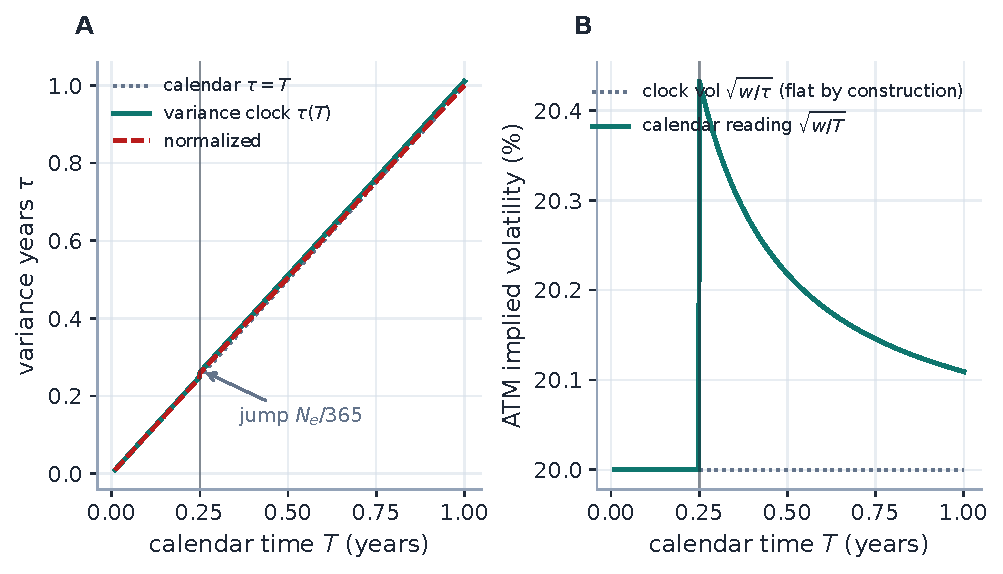
\includegraphics[width=\textwidth]{fig_emc_clock.pdf}
\caption{Two clocks, one set of prices (production clock code).  A: the
variance clock \eqref{eq:clock} jumps $N_e/365$ at the event; the
normalized variant (dashed) rescales so the one-year budget is
unchanged.  B: the same total-variance curve read two ways --- flat
against its own clock, the familiar event hump against the calendar.
The hump is a property of the ruler, not of the prices.}
\label{fig:clock}
\end{figure}

The clock is a few lines, verified against production to \emcrefagree\
(\cref{app:ref}):

\begin{lstlisting}[caption={The event variance clock \eqref{eq:clock}
(distilled from \texttt{calib/weighted\_time.py}).},label={lst:clock}]
def weighted_variance_years(t_cal, events, normalize=False, dpy=365.0):
    if t_cal <= 0: return t_cal        # events: (t_e, N_e), N_e = EXTRA days
    tau_days = t_cal*dpy + sum(N for te, N in events if te <= t_cal and N > 0)
    if normalize:                      # rescale so a 1Y budget stays dpy days
        e1 = sum(N for te, N in events if te <= 1.0 and N > 0)
        tau_days *= dpy/(dpy + e1)
    return tau_days/dpy                # tau(T); equals t_cal with no events
\end{lstlisting}

\subsection{Normalization: fixing the year's budget}

Un-normalized, the cumulative weight exceeds the day count
($\tau>T$).  The normalization toggle rescales \emph{all} days by one
factor so the one-year budget stays $365$:
\begin{equation}
\tau_{\mathrm{days}}(T)\ \longmapsto\
\tau_{\mathrm{days}}(T)\cdot\frac{365}{365+\sum_{t_e\le1}N_e} .
\label{eq:normalize}
\end{equation}
Then the one-year variance time --- and the one-year implied vol ---
match a no-event year exactly: events \emph{redistribute} variance
within the year rather than add it.  Which convention to run is a desk
choice, not a mathematical one: un-normalized treats events as
genuinely extra variance against a one-per-day baseline; normalized
treats the year's budget as known and the events as its scheduled
lumps.  Exercise~3 computes what normalization does to the sub-year
readings.

\paragraph{Exercise 1.}
Derive \eqref{eq:crush} from \cref{prop:gauge}(iii) and evaluate it for
the worked event: $T=0.30$, $N_e=4$, so
$\tau=\emctauprobe$.  Confirm the \emcdropbp-vol-bp drop at
$\sigma_{\mathrm{cal}}=20\%$, and note the crush scales like
$N_e/(2\cdot365\,T)$ for small events --- steepest for the shortest
expiries, exactly where desks watch it.

%======================================================================
\section{Reading the clock off prices}
\label{sec:read}

Everything so far ran the clock forward: given a calendar, re-read the
surface.  The productive direction is backwards: the market's prices
carry information about the clock, and two production mechanisms
extract it.

\subsection{Interpolate in the clock, not in the calendar}

Between quoted expiries the term view needs a dense curve.  The
production rule interpolates total variance \emph{linearly in $\tau$}
--- constant forward variance per unit of the market's clock, the
discrete restatement of ``Brownian on its own clock'' --- with
rate-preserving extrapolation at both ends.  \Cref{fig:interp} is the
wrong-way demo: on quotes generated by a flat clock vol around one
event, the production interpolation reproduces the flat-then-hump
reading exactly, while the calendar-clock interpolation smears the
event's variance across the whole bracketing interval --- a
\emcinterpgapbp-vol-bp artifact at expiries nobody quotes, largest just
before the event where a desk would price an event-straddle off the
dense curve.

\begin{figure}[H]
\centering
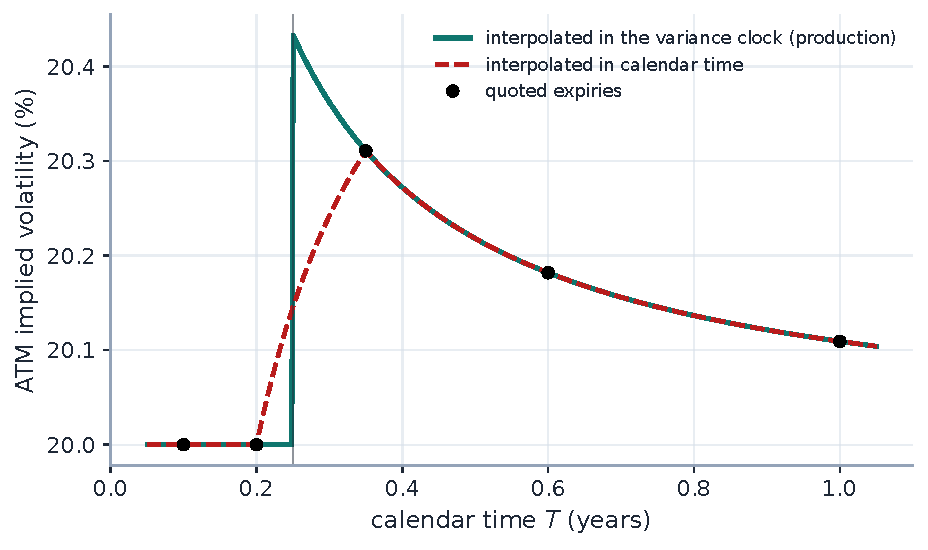
\includegraphics[width=0.86\textwidth]{fig_emc_interp.pdf}
\caption{Interpolate in the clock, not the calendar (production
interpolator both ways).  Quotes (dots) are generated by a flat vol on
the event clock.  Linear-in-$\tau$ interpolation (teal) reproduces the
true reading: flat to the event, the jump, the decay.  Linear-in-$T$
interpolation (dashed) smears the event's variance across the
bracketing interval --- up to \emcinterpgapbp\ vol bp of phantom vol at
unquoted maturities.  The event sits \emph{between} quotes; only the
clock knows it is there.}
\label{fig:interp}
\end{figure}

\subsection{The auto-calibrator: an inverse problem with a sparsity prior}

The calendar need not be typed in.  The term workspace's auto-calibrate
action infers it from the ATM term structure: place one candidate event
before each quoted expiry up to a chosen horizon, and solve for
non-negative extra days $\{N_i\}$ minimizing
\begin{equation}
J(N)=\sum_i\big(f_{i+1}-f_i\big)^{2}
+\lambda_{\mathrm{mono}}\sum_i\big(\min(f_{i+1}-f_i,0)\big)^{2}
+\lambda_{1}\sum_i\frac{N_i}{365}
+\lambda_{2}\sum_i\Big(\frac{N_i}{365}\Big)^{2},
\label{eq:autocal}
\end{equation}
where $f_i=\Delta \tvar_i/\Delta\tau_i(N)$ is the \emph{event-time}
forward variance of interval $i$ (a bounded quasi-Newton solve; events
under half a day are thresholded away; the first interval past the
horizon carries no candidate and anchors the tail).  Three structural
facts make \eqref{eq:autocal} sound.  The calendar-time forward
variance is event-\emph{invariant} --- prices fix $\tvar$
(\cref{prop:gauge}) --- so the objective must work on the dilated
clock, the only one events move.  An event can only \emph{lengthen} its
interval's weighted time, so it can only pull a forward-variance spike
\emph{down} toward its neighbours: the solver reads the calendar off
exactly the kinks the clock was built to explain.  And the asymmetric
monotonicity term spends its budget on \emph{decreases} of forward
variance --- the shape a genuine pre-event interval produces --- rather
than on an ordinary upward-sloping term structure.

What can such an estimator promise?  \Cref{fig:ident} is the audit.  At
single-name vol ($40\%$) a planted event is recovered at the correct
interval to within \emcidentshrink\ extra days across sizes ---
the small downward bias is the $\ell_1$ term's shrinkage, the standard
price of a sparsity prior.  At index vol ($20\%$) the same planted
events sit \emph{below the solver's materiality threshold} up to
\emcidentlowfloor\ extra days: the flatness gain a small event offers
scales with $\sigma^{4}$ while the sparsity charge does not, so quiet
names keep empty calendars unless the kink is large --- a deliberate
design, not a failure.  A flat term structure returns exactly
\emcidentflat\ events.

\begin{figure}[H]
\centering
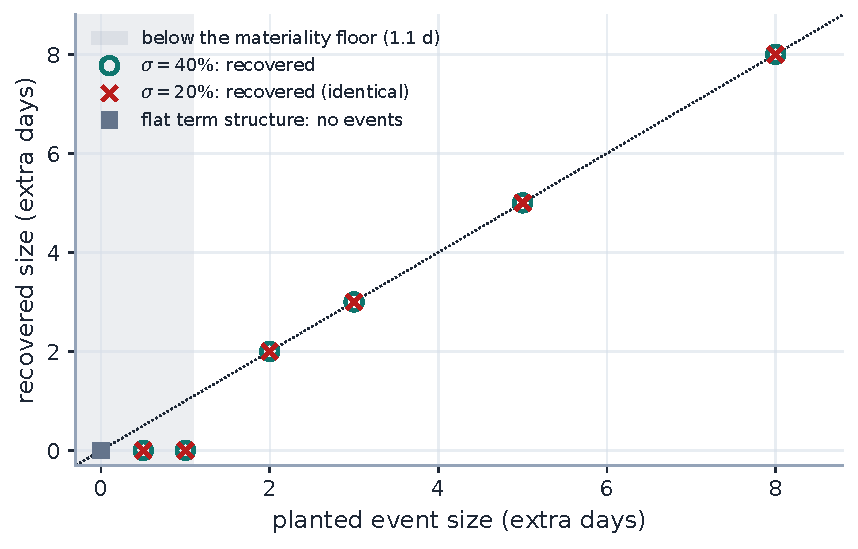
\includegraphics[width=0.80\textwidth]{fig_emc_ident.pdf}
\caption{What the inverse problem can promise (production solver).
Planted events are recovered on the diagonal at single-name vol, with
the $\ell_1$ shrinkage visible as a downward bias of at most
\emcidentshrink\ days; at index vol the same events fall below the
materiality threshold until they are large --- the sparsity prior
working as designed.  A flat term structure solves to an empty
calendar.}
\label{fig:ident}
\end{figure}

\subsection{Reading a live clock: AAPL}

\Cref{fig:hero} runs the production solver on the real AAPL term
structure of the standing export (\emcheronodes\ expiries, valuation
date 2026-07-18).  Per \emph{calendar} year, the forward-variance
ladder is uneven --- the interval containing the late-October earnings
runs visibly hot.  The solver installs \emcheroeventcount\ events worth
\emcherodays\ extra days in total, the bulk against the
earnings-bearing interval, and the ladder's spread tightens from
\emcherospreadbefore\ to \emcherospreadafter\ variance bp.  Two honest
readings of that exhibit.  The solver has recovered, from prices alone,
that this interval contains materially more than its share of calendar
days' variance --- the market's clock runs fast through it.  But the
solver cannot \emph{name} the reason: it reads kinks, and every source
of elevation --- earnings, a macro date, genuine term-structure shape
--- looks identical through \eqref{eq:autocal}.  The installed calendar
is an estimate to be reviewed and edited in the term workspace, not an
oracle (\cref{sec:limits}).

\begin{figure}[H]
\centering
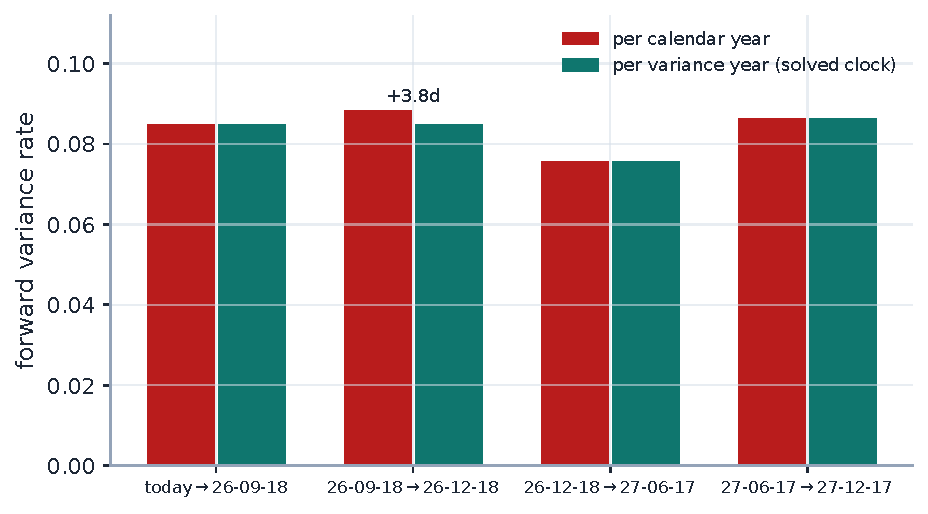
\includegraphics[width=0.86\textwidth]{fig_emc_hero.pdf}
\caption{Reading the clock off live AAPL (production solver on the
standing export's term structure).  Per calendar year (rust) the
earnings-bearing interval runs hot; the solver installs
\emcherodays\ extra days (annotated), and per variance year (teal) the
ladder flattens --- forward-variance spread \emcherospreadbefore\ to
\emcherospreadafter\ variance bp.  The market's clock runs fast through
that interval; the solver measures by how much, not why.}
\label{fig:hero}
\end{figure}

\paragraph{Exercise 2.}
Prove the within-interval non-identifiability: the fits and every
consumer read the clock only through $\tau$ at the quoted maturities
\eqref{eq:clock}, which depends on the calendar only through the
cumulative sums $\sum_{t_e\le T_i}N_e$.  Conclude that two events
inside the same quoted interval are indistinguishable from one event of
their combined size anywhere in that interval --- which is why the
solver's midpoint placement is a convention, not an estimate --- and
that an event's \emph{date} becomes identified only when an expiry is
listed between it and its neighbours.

\paragraph{Exercise 3.}
With normalization on \eqref{eq:normalize} and the worked calendar (one
event, $N_e=4$, $t_e=\emcte$), compute the working vol of a six-month
expiry relative to the un-normalized clock, and verify the one-year
reading is exactly the no-event one.  Then say in one sentence why
normalization cannot affect the auto-calibrator's solved events (hint:
one global factor cancels in every forward-variance ratio the flatness
term compares).

%======================================================================
\section{One clock through the whole pipeline}
\label{sec:thread}

The clock is computed once per node --- $\tau$ is stored beside the
calendar maturity in the prepared quotes, and folded into the fit cache
key --- and every consumer reads that one number: the parametric and
local-vol fits, the vol$\leftrightarrow$variance conversions (including
Note~08's var-swap targets), the term structure, the option table, and
the 3-D surface mesh, which is quoted in $\sqrt{\tvar/\tau}$ and
carries both clocks so a stacked view can recover price variance
(invariant~3; a surface tab reading the calendar clock while the smile
read the variance clock was a real, test-locked regression).  Editing a
calendar bumps a per-ticker events version, so one name's earnings
entry never refits the rest of the universe (invariant~4); an empty
calendar short-circuits to $\tau=T$ and the pipeline is byte-identical
(invariant~2).

\begin{remark}[One production clock, one legacy clock, one unit trap]
\label{rem:twoclocks}
Two dilation clocks exist in the codebase and must not be conflated.
The production clock is \eqref{eq:clock} --- day-weighted, the one
every fit and view consumes, including the production term-structure
interpolator of \cref{sec:read}.  The older \texttt{EventClock}
survives only in its own tests: it predates the day convention (its
weights are \emph{years} of equivalent diffusion time) and its
interpolation method is the historical ancestor of the shipped one.
Hence the unit trap: an event's \texttt{weight} is \emph{extra
equivalent days}, never years --- the schema docstring said years until
2026-07-09 and the legacy module's comments remain the stale party.
When in doubt, the production semantics is the one \cref{lst:clock}
and its tests lock.
\end{remark}

\begin{remark}[The intraday hook, and the other clock in the building]
\label{rem:intraday}
Two refinements post-date the original design.  First, the clock's base
need not be the calendar-day count: an intraday session profile can
supply the accrued day-weight while the event cutoff stays on calendar
time, which makes a \emph{fractional} event date meaningful --- an
08:30 CPI print is now a genuine intraday event.  Second, the
observation filter of Note~15 carries its own \emph{session clock} for
a different question entirely: how much handle drift to expect
\emph{between two snapshots} (a weekend moves ATM like one overnight).
That clock budgets process noise between fits; this note's clock
dilates maturity within one fit.  They share the intraday primitive and
nothing else --- separate toggles, separate subsystems, no
interaction.
\end{remark}

%======================================================================
\section{What is genuinely original here}
\label{sec:original}

Time changes are classical (Bergomi dilates around events; An\'e and
Geman read equity returns as Brownian on a transaction clock).  The
contributions are the engineering shape.  \emph{Price preservation by
construction}: the clock enters only as a denominator, so the invariance
column of \cref{prop:gauge} is arithmetic, not a property to defend ---
adding an event can never move a price or create arbitrage.  \emph{The
day-weighted parametrization}: one intuitive number per event (extra
equivalent days) a desk can quote, with the normalization
\eqref{eq:normalize} cleanly separating ``extra variance'' from
``reallocated budget.''  \emph{The solver as a disciplined inverse}:
flatten event-time forward variance under a sparsity prior, with the
identifiability limits measured rather than hidden
(\cref{fig:ident}) --- shrinkage quantified, materiality threshold
explicit, flat input provably eventless.  And the byte-identical empty
calendar makes the whole feature strictly additive.  The payoff is
comparability: pre- and post-earnings surfaces line up across names and
dates because event-time vol is the signal --- calendar-time vol is the
artifact.

%======================================================================
\section{Limitations}
\label{sec:limits}

Where the guarantees stop.  \emph{The clock is deterministic}: it
forecasts the schedule of $\qv{M}$, not its randomness --- no
vol-of-vol, no stochastic event size; that is model territory (Bergomi
\cite{Bergomi2016}), deliberately out of scope.  \emph{Events must be
scheduled}: an unscheduled jump is not a clock feature, and the crush
factor \eqref{eq:crush} prices only the anticipated part.  \emph{The
solver reads ATM only}: the auto-calibrator consumes the ATM
total-variance ladder; the smile's event signature (strangle richness)
is unused information.  \emph{Placement is a convention}: within a
quoted interval an event's date is unidentified (Exercise~2), and the
midpoint is a choice.  \emph{Sizes are shrunk and thresholded}: the
$\ell_1$ prior biases solved days downward by up to
\emcidentshrink\ on the audit and zeroes sub-materiality events
entirely on quiet names (\cref{fig:ident}) --- review the installed
calendar rather than trusting it.  \emph{Kinks have no fingerprint}:
the solver cannot distinguish an earnings kink from genuine
term-structure shape (the AAPL exhibit's honest reading).  And
\emph{normalization is a convention}, not an inference: it changes
every sub-year reading while leaving prices, fits and solved events
untouched.

\appendix
%======================================================================
\section{Hyperparameter atlas}
\label{app:atlas}

The only home for settings names: the body speaks mathematics, this
table speaks configuration.

\begin{longtable}{p{0.28\textwidth}p{0.14\textwidth}p{0.50\textwidth}}
\caption{Event-clock hyperparameters.}\label{tab:atlas}\\
\toprule Knob & Default & Role\\ \midrule
\endfirsthead \toprule Knob & Default & Role\\ \midrule \endhead
\multicolumn{3}{l}{\emph{Surfaced}}\\ \midrule
\texttt{eventsEnabled} & \texttt{true} & Master toggle: off forces
$\tau=T$ everywhere.\\
\texttt{normalizeEvents} & \texttt{false} & The one-year budget
normalization \eqref{eq:normalize}.\\
per-ticker calendar & empty & \texttt{EventSpec}$(t_e>0,\ N_e\ge0,$
label$)$, $N_e$ in \emph{extra equivalent days}; persisted per ticker
(its own endpoint and version), not in the global options.\\
\texttt{maxExpiry} & --- & Auto-calibrate horizon (per request): one
candidate event per expiry at or before it.\\
\midrule
\multicolumn{3}{l}{\emph{Hidden}}\\ \midrule
\texttt{DAYS\_PER\_YEAR} & $\emcdays$ & Calendar-to-variance day
conversion.\\
\texttt{mono\_weight} & $1.0$ & Auto-calibrate penalty on
\emph{decreasing} event-time forward variance \eqref{eq:autocal}.\\
\texttt{sparse\_weight} / \texttt{ridge\_weight} & $10^{-3}$ /
$10^{-4}$ & The $\ell_1$/$\ell_2$ priors keeping solved events small
and sparse.\\
\texttt{min\_event\_days} & $0.5$ & Sparsity threshold: smaller solved
events are dropped.\\
\texttt{max\_event\_days} & $1825$ & Solver box bound per event.\\
\texttt{base\_days} & \texttt{None} & Intraday hook: session-profile
day-weights replace the calendar base (\cref{rem:intraday}).\\
\bottomrule
\end{longtable}

\noindent\textbf{Performance.}  The clock is a scalar sum per node ---
negligible; with no events $\tau=T$ and the feature costs exactly
nothing.  The auto-calibrator is one bounded quasi-Newton solve over a
handful of variables, interactive.  A calendar edit refits one ticker
(per-ticker events version in the fit key).

%======================================================================
\section{Traceability}
\label{app:trace}

\begingroup
\small
\setlength{\tabcolsep}{4pt}
\renewcommand{\arraystretch}{1.15}
\begin{longtable}{@{}p{0.42\textwidth}p{0.10\textwidth}p{0.44\textwidth}@{}}
\caption{Claims in this note and the code/tests that lock them.}
\label{tab:trace}\\
\toprule Claim & Object & Code anchor \newline \emph{Test anchor}\\ \midrule
\endfirsthead
\toprule Claim & Object & Code anchor \newline \emph{Test anchor}\\ \midrule
\endhead
No events: identity clock, byte-identical pipeline &
invariant~2 &
\nolinkurl{volfit/calib/weighted_time.py}\newline
\nolinkurl{tests/test_weighted_time.py::test_no_events_is_identity};
\nolinkurl{::test_no_event_byte_identical}\\
\addlinespace
Event adds day weights before its date only &
\eqref{eq:clock} &
\nolinkurl{volfit/calib/weighted_time.py}\newline
\nolinkurl{tests/test_weighted_time.py::test_event_before_adds_day_weights}\\
\addlinespace
Price preservation: readings scale by $\sqrt{T/\tau}$, LV included &
\eqref{eq:crush} &
\nolinkurl{volfit/api/service.py},
\nolinkurl{volfit/api/displayed.py}\newline
\nolinkurl{tests/test_weighted_time.py::test_event_lowers_iv_by_sqrt_t_over_tau};
\nolinkurl{::test_localvol_iv_drops_with_event}\\
\addlinespace
Normalization pins the one-year budget &
\eqref{eq:normalize} &
\nolinkurl{volfit/calib/weighted_time.py}\newline
\nolinkurl{tests/test_weighted_time.py::test_normalization_pins_one_year};
\nolinkurl{::test_normalization_keeps_one_year_vol}\\
\addlinespace
Surface mesh shares the smile's clock &
\cref{sec:thread} &
\nolinkurl{volfit/api/affine_views.py},
\nolinkurl{volfit/api/surface.py}\newline
\nolinkurl{tests/test_surface_clock.py::test_surface_mesh_uses_variance_clock_like_the_smile}\\
\addlinespace
Dilated interpolation recovers lumped event variance; legacy clock
confined to its tests &
\cref{fig:interp} &
\nolinkurl{volfit/calib/weighted_time.py},
\nolinkurl{volfit/calib/event_time.py}\newline
\nolinkurl{tests/test_event_time.py::test_interpolation_lumps_event_variance}\\
\addlinespace
Auto-calibrate flattens the dilated forward variance; flat input stays
eventless; horizon respected; endpoint installs the shared calendar &
\eqref{eq:autocal} &
\nolinkurl{volfit/calib/event_autocalib.py},
\nolinkurl{volfit/api/event_autocalib.py}\newline
\nolinkurl{tests/test_event_autocalib.py::test_spike_is_flattened};
\nolinkurl{::test_flat_input_stays_eventless};
\nolinkurl{::test_horizon_limits_events};
\nolinkurl{::test_autocalibrate_endpoint_sets_calendar}\\
\bottomrule
\end{longtable}
\endgroup

%======================================================================
\section{Reference implementation}
\label{app:ref}

\Cref{lst:clock} was executed against the production
\texttt{weighted\_variance\_years} by this edition's generator on every
run --- both normalization settings, a four-event calendar, maturities
to two years --- agreeing to \emcrefagree\ (floating-point identity).
The production module also carries the dense-curve interpolator used in
\cref{fig:interp} (linear in $\tau$, rate-preserving beyond the quoted
ends); the figure exercises the shipped function on both clocks rather
than reimplementing either.

\begin{thebibliography}{9}
\bibitem{Dambis1965} K.~Dambis.  On the decomposition of continuous
submartingales.  \emph{Theory Probab.\ Appl.}, 10:401--410, 1965.
\bibitem{DubinsSchwarz1965} L.~Dubins and G.~Schwarz.  On continuous
martingales.  \emph{Proc.\ Nat.\ Acad.\ Sci.}, 53:913--916, 1965.
\bibitem{AneGeman2000} T.~An\'e and H.~Geman.  Order flow, transaction
clock, and normality of asset returns.  \emph{J.\ Finance},
55(5):2259--2284, 2000.
\bibitem{Bergomi2016} L.~Bergomi.  \emph{Stochastic Volatility
Modeling}.  CRC Press, 2016.
\bibitem{Gatheral2006} J.~Gatheral.  \emph{The Volatility Surface}.
Wiley, 2006.
\end{thebibliography}

\end{document}
